\section{Amplificatore differenziale e mediatore}

Si è proceduto a montare il circuito in \fig{ampli_media}, il valore misurato dei componenti utilizzati è riportato a lato.

\begin{figure}[H]
	\begin{minipage}{0.75\textwidth}
		\centering
		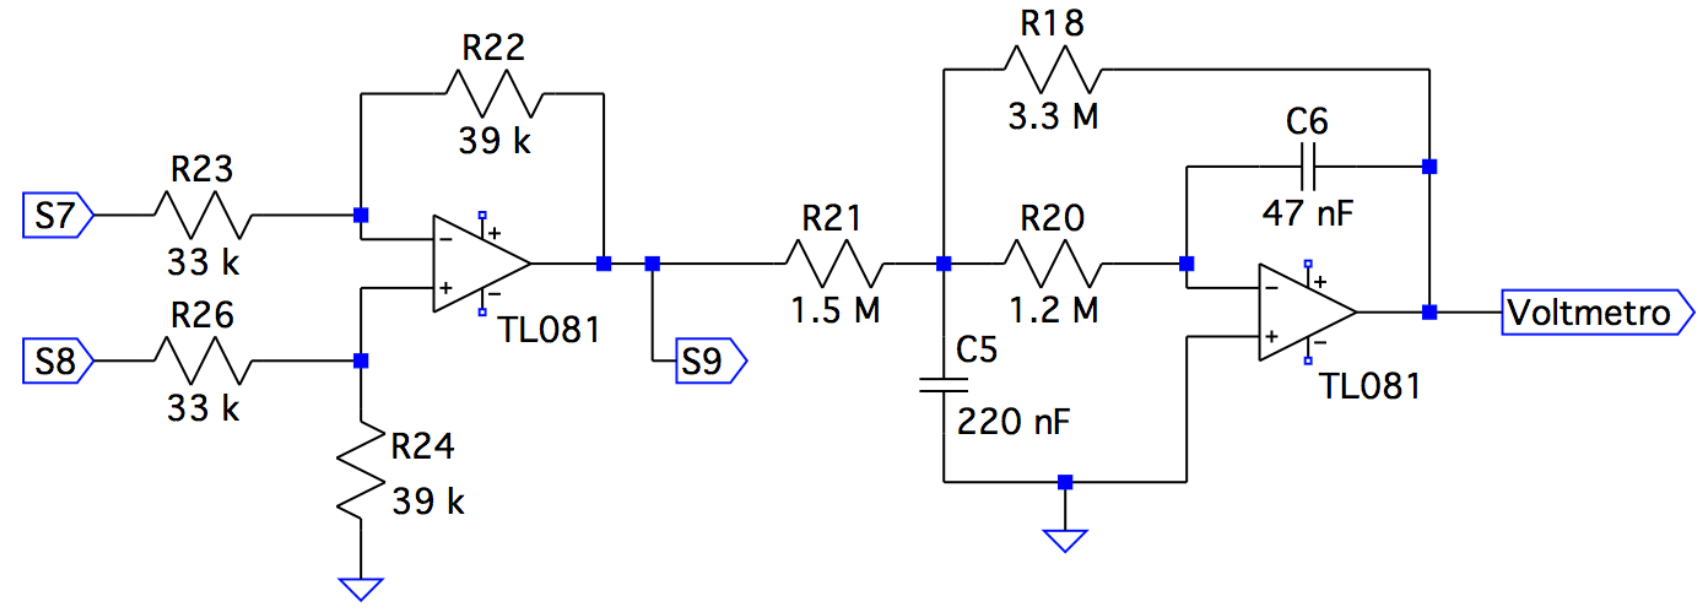
\includegraphics[width=1\textwidth]{ampli_media.png}
		\caption{Schema dell'amplificatore differenziale in serie al mediatore}
		\label{fig:ampli_media}
	\end{minipage}
	\begin{minipage}{0.19\textwidth}
		\begin{tabular}{l@{ }c@{ }l}
			$R_{18}$& = &\SI{3.19(4)}{\mega\ohm}\\
			$R_{20}$& = &\SI{1.22(1)}{\mega\ohm}\\
			$R_{21}$& = &\SI{1.45(1)}{\mega\ohm}\\
			$R_{22}$& = &\SI{38.2(4)}{\kilo\ohm}\\
			$R_{23}$& = &\SI{32.5(4)}{\kilo\ohm}\\
			$R_{24}$& = &\SI{38.3(4)}{\kilo\ohm}\\
			$R_{26}$& = &\SI{32.0(4)}{\kilo\ohm}\\
			$C_5$& = &\SI{228(9)}{\nano\farad}\\
			$C_6$& = &\SI{51(2)}{\nano\farad}
		\end{tabular}
	\end{minipage}
\end{figure}

\paragraph{Amplificatore differenziale} La prima parte del circuito è un amplificatore differenziale che prende in ingresso le uscite $S7$ e $S8$ e in uscita ($S9$) e in condizioni ideali restituisce la differenza amplificata di un fattore $g_f$ (guadagno differenziale).
In particolare se $R_{23} = R_{26}$ e $R_{22} = R_{24}$\footnote{In realtà basterebbe fossero proporzionali}, allora la tensione in uscita sarà: $$V_{S9}=(V_{S8}-V_{S7})\frac{R_{23}}{R_{22}}$$ dove perciò è presente solo amplificazione differenziale e non amplificazione di modo comune.

Come misurato, le resistenze non sono esattamente uguali, perciò il comportamento devierà leggermente da quello ideale, in particolare ci attendiamo che $$V_{S9}=V_{S8}\frac{R_{23}}{R_{23}+R_{22}}\frac{R_{24}}{R_{24}+R_{26}}-V_{S7}\frac{R_{22}}{R_{23}}$$, in particolare i guadagni di modo comune e differenziale saranno:

$$A_d = \frac{1}{2}\frac{R_{23}+R_{22}}{R_{23}}\frac{R_{24}}{R_{24}+R_{26}} + \frac{1}{2}\frac{R_{22}}{R_{23}} = 1.180\pm0.011$$
$$A_c = \frac{1}{2}\frac{R_{23}+R_{22}}{R_{23}}\frac{R_{24}}{R_{24}+R_{26}} - \frac{1}{2}\frac{R_{22}}{R_{23}} = 0.005\pm0.005$$

Considerato il segnale in ingresso, l'uscita in condizioni ideali sarà il segnale originale al quale è stata invertita un semi-onda. La posizione della semi-onda invertita cambierà in base alla posizione del deviatore: il segnale in ingresso all'amplificatore varia come in \fig{S7a} (segnale diretto) e \fig{S7b} (segnale sfasato di 90°). L'uscita dell'amplificatore differenziale nei due casi è riportata di seguito in \fig{S9a} e \fig{S9b}.

Si verifica che nel primo caso il segnale è sempre negativo, mentre nel secondo è sostanzialmente a media nulla, come atteso.

Essendo presente un guadagno di modo comune, seppur piccolo, il risultato sarà un'asimmetria nelle due semi-onde, come in effetti si osserva\footnote{Questo non è l'unico motivo per cui aspettarsi una asimmetria tra le due semi-onde, c'è infatti da considerare la risposta del fotodiodo, possibilmente non lineare.}.

\begin{figure}[h]
		\centering
		\subfloat[Deviatore collegato a $S1$]{
			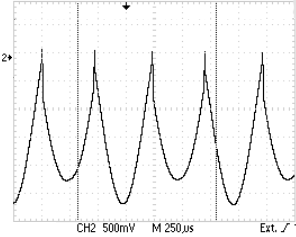
\includegraphics[scale=0.8]{s9a.png}
			\label{fig:S9a}
		}
		\subfloat[Deviatore collegato ad $S2$]{
			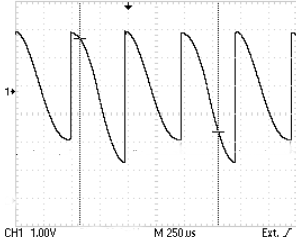
\includegraphics[scale=0.8]{s9b.png}
			\label{fig:S9b}
		}
		\caption{Segnali acquisiti su $S_9$}
		\label{fig:s7}
\end{figure}

\paragraph{Mediatore} La seconda parte del circuito è un mediatore che prende in ingresso l'uscita $S9$ dell'amplificatore differenziale e restituisce in output il valore medio.

Misurando con il voltmetro l'output quando il deviatore è su $S2$, quindi il segnale in ingresso è quello in \fig{S9b}, il valore letto è dell'ordine di qualche decina di $\si{\milli\volt}$. Agendo sul potenziometro per la regolazione della fase è possibile calibrare il circuito in modo che la media sia il più possibile vicina a 0.

Portando adesso il deviatore su $S1$ in output avremo il valore di tensione che ci interessa per la misura dell'assorbimento del mylar.

Il mediatore si comporta sostanzialmente come un filtro passa basso, in \fig{bode} è riportato il diagramma di Bode di questo circuito, che ha quindi una frequenza di taglio di $\sim\SI{0.5}{\hertz}$.

\begin{figure}[h]
	\centering
	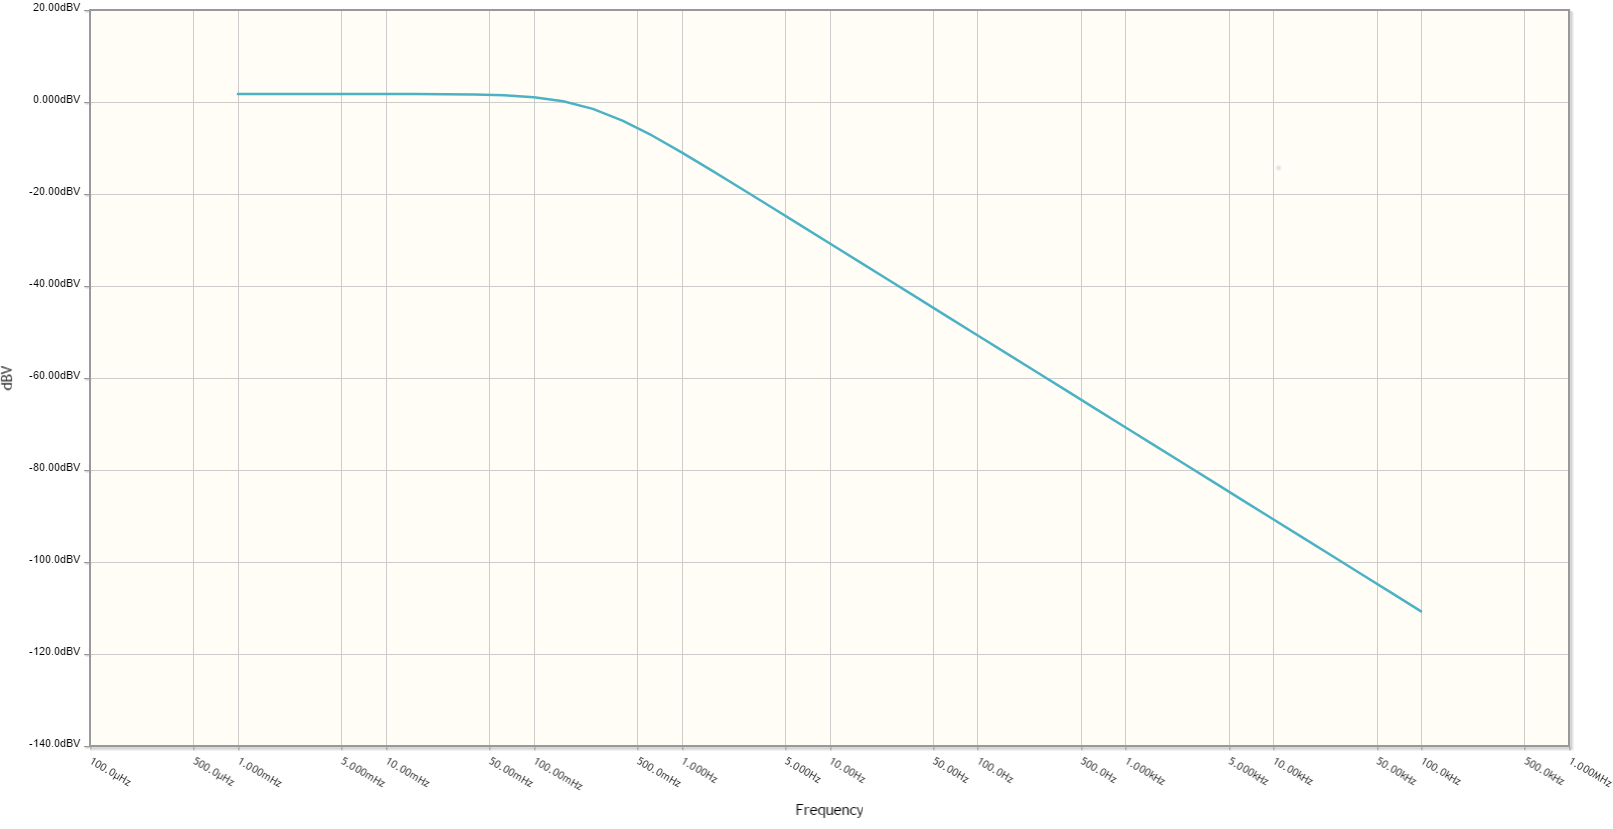
\includegraphics[scale=0.2]{bode.png}
	\caption{Diagramma di Bode del mediatore}
	\label{fig:bode}
\end{figure}


\section{Misura della costante di assorbimento}
Si è proceduto quindi alla misura finale, obiettivo di questa esperienza: si sono posizionate delle lastrine di mylar tra il LED e il fotodiodo e si è registrato il valore di tensione in uscita al variare del numero di lastrine. I dati raccolti sono riportati in \tab{data}.

Dove il valore di tensione non fosse stato stabile all'ultima cifra, si è proceduto a stimare l'incertezza della misura in base al range di oscillazione.

Durante queste misure si è verificato che il circuito è poco sensibile al rumore ambientale (in particolare le luci della stanza, che oscillano con una frequenza di \SI{100}{\hertz}), infatti coprendo il circuito (isolandolo dalla luce ambientale) il valore letto rimane sostanzialmente immutato.

Si è proceduto quindi al fit della legge di assorbimento esponenziale $V = V_0 \cdot e^{n/k}+a$, dove $k$ è la costante di assorbimento\footnote{In unità di spessore di una lastra: $\sim\SI{150}{\micro\meter}$.} e si è valutato di aggiungere una costante $a$ per stimare l'offset dovuto alla non perfetta calibrazione dello 0\footnote{Per quanto calibrato alla sezione precedente, lo 0 dipende in maniera non trascurabile dalle posizioni reciproche di LED e diodo. Questo comportamento non dovrebbe avvenire in un circuito ideale ed è probabilmente dovuto all'asimmetria del segnale all'ingresso del mediatore, come visto in \fig{S9a}: piccoli spostamenti del LED potrebbero (e probabilmente hanno) modificato lo 0.}.

Il numero di lastre è un numero intero, tuttavia non è nota l'incertezza sullo spessore delle stesse. Considerati i piccoli errori sulle tensioni, un errore dell'ordine del $\sim 1\%$ è importante nel calcolo del $\chi^2$.
Nell'analisi si è valutato di scartare le prime 3 misure poiché evidentemente outlier, probabilmente dovuti ad un piccolo spostamento del LED.

I risultati del fit eseguito sono:
$$V_0 = \SI{2.11 \pm 0.04}{\volt} \qquad k = 5.71 \pm 0.24 \qquad a = \SI{-0.117 \pm 0.021}{\volt}$$
$$ \text{corr}(V_0,k) = -0.79 \qquad \text{coor}(V_0,a) = 0.63 \qquad \text{corr}(k,a) = -0.97$$

Il valore del $\chi^2$ dipende fortemente dalla presenza o meno dell'errore sullo spessore delle lastre. Nell'ipotesi che questo sia trascurabile $\chi^2 /\text{ndof} = 30.3 / 8$, con un $p = 0.02\%$. Se invece, ad esempio, l'errore sullo spessore è $1\%$ si ottiene $\chi^2 /\text{ndof} = 10.2 / 8$ e un $p = 25.0\%$, che sembra quindi ragionevole.

Il grafico dei dati e del fit realizzato è riportato in \fig{fit}.

\begin{figure}[H]
		\begin{minipage}{0.28\textwidth}
			\begin{tabular}{cc}
				\toprule
				\# lastre & Tensione [V]\\
				\midrule
				0  & 2.05 $\pm$ 0.02\\
				1  & 1.495 $\pm$ 0.022\\
				2  & 1.214 $\pm$ 0.018\\
				3  & 1.137 $\pm$ 0.017\\
				4  & 0.915 $\pm$ 0.014\\
				5  & 0.770 $\pm$ 0.012\\
				6  & 0.636 $\pm$ 0.010\\
				7  & 0.514 $\pm$ 0.008\\
				8  & 0.397 $\pm$ 0.006\\
				9  & 0.306 $\pm$ 0.005\\
				10 & 0.249 $\pm$ 0.004\\
				11 & 0.203 $\pm$ 0.003\\
				12 & 0.1405 $\pm$ 0.0021\\
				13 & 0.1000 $\pm$ 0.0015\\
				\bottomrule
			\end{tabular}
			\captionof{table}{Dati raccolti}
			\label{tab:data}
		\end{minipage}
	\begin{minipage}{0.75\textwidth}
		\centering
		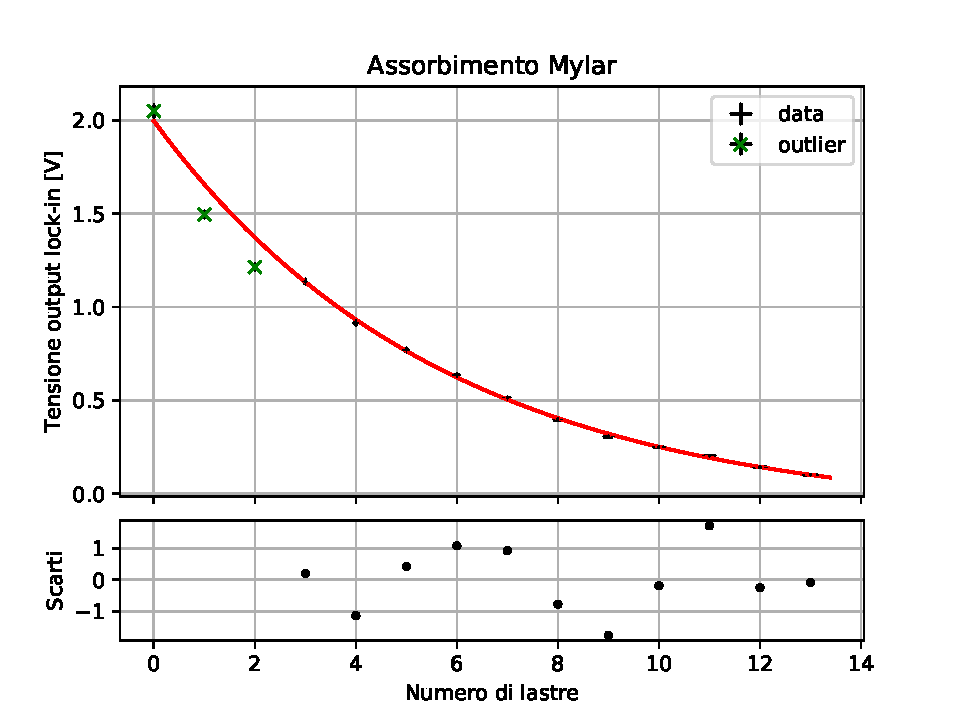
\includegraphics[width=1.05\textwidth]{fit_data.pdf}
		\caption{Fit della legge di assorbimento}
		\label{fig:fit}
	\end{minipage}
\end{figure}
